\documentclass[a4paper,11pt]{article}
\usepackage[utf8]{inputenc}
\usepackage[francais]{babel}
\usepackage[T1]{fontenc}

\usepackage[toc,page]{appendix}
%fonts pour les math
\usepackage{amsfonts}
\usepackage{amsmath}
\usepackage{dsfont}
%couleur dans le doc
\usepackage[dvipsnames]{xcolor}

\usepackage{enumitem}
\frenchbsetup{StandardLists=true}
\usepackage{multirow}
\usepackage{hyperref}

%affichage lignes de code
\usepackage{listings}
\usepackage{textcomp}
\lstset{
	tabsize=2,
	language=python,
        basicstyle=\scriptsize,
        upquote=true,
        aboveskip={0.2\baselineskip},
        columns=fixed,
        showstringspaces=false,
        extendedchars=true,
        breaklines=true,
        prebreak = \raisebox{0ex}[0ex][0ex]{\ensuremath{\hookleftarrow}},
        frame=single,
        showtabs=false,
        showspaces=false,
        showstringspaces=false,
        identifierstyle=\ttfamily,
        keywordstyle=\color[rgb]{0,0,1},
        commentstyle=\color[rgb]{0.133,0.545,0.133},
        stringstyle=\color[rgb]{0.627,0.126,0.941},
}

%\usepackage{lastpage}
%pour les images
	\usepackage[dvips, pdftex]{graphicx}
	\usepackage[section]{placeins}
	\usepackage{here}	
	\usepackage{float}

%définition du titre du document
 \newcommand{\titleinfo}{INF441-NET - NetProbes} 

%formattage de la page
	\usepackage{geometry}
	\geometry{top=2cm, bottom=2cm, left=2cm, right=2cm}
	%fomattage de l'entête et du pied de page
	\usepackage{fancyhdr}
	\pagestyle{fancy}
		\setlength{\headheight}{15.2pt}
		\lhead{\titleinfo\\}
		\rhead{\leftmark}
	%Page de garde avec style vide
	\thispagestyle{empty}	
	

%formattage du titre des sections
	%\usepackage{titlesec}
	%\titleformat{\section}[runin]{\normalfont\bfseries}{\sectionprefix \thesection}{1pt}{}[.]

%longueur des sauts de paragraphe
\setlength{\parskip}{1ex}

%commande pour les ensembles
\newcommand{\R}{\mathbb{R}}
\newcommand{\N}{\mathbb{N}}
\newcommand{\C}{\mathbb{C}}
\newcommand{\cd}[1]{\texttt{#1}}

%commande pour les notations de map
	%\newcommand{\I}{\mathds{1}}
	%\newcommand{\p}{\mathds{P}}
	%\newcommand{\E}{\mathds{E}}
	%\renewcommand{\P}{\mathds{P}}


%commande pour les opérateurs
\newcommand{\INT}{\displaystyle\int}
\newcommand{\SUM}{\displaystyle\sum}
\newcommand{\FRAC}{\displaystyle\frac}
\newcommand{\PROD}{\displaystyle\prod}
\newcommand{\INF}{\displaystyle\inf}

%commande pour environnement description
\newcommand{\desc}[1]{\item[] \texttt{#1}}
\usepackage{hyperref}
\hypersetup{
    colorlinks,
    citecolor=black,
    filecolor=black,
    linkcolor=black,
    urlcolor=black
}

\begin{document}

\thispagestyle{empty}							%page de garde vide
%\begin{document}
	\begin{center}
		\hfill
		François \bsc{Espinet}
		\hfill \hfill
		Gaspard \bsc{Ferey}
		\hfill ~
		\par
		\noindent
		\\
		\vspace{0.7cm}
		\textit{Promotion X2011}
		\vfill\vfill
		\Huge
		\begin{tabular}{c}
			\hline
			%Projet\\
			NetProbes\\
			{\Large{\textsc{~~~~~INF441-NET~~~~~}}}\\
			\hline
		\end{tabular}
		\large
		\vfill
		Diagnostics réseau distribués
	\end{center}
	\vfill
	\begin{flushright}
	
\includegraphics[scale=0.1]{img/logo_x.png}
	\end{flushright}
	\newpage 


\tableofcontents

\section{NetProbes : un programme de diagnostic réseau distribué}
Le but de ce programme est de permettre d'effectuer des tests sur un réseau donné.

Après avoir établi un réseau de sondes au-dessus du réseau test via http, on pourra lancer les tests de notre choix sur ce réseau et collecter les résultats pour analyse.

L'architecture de l'application nous permet d'implémenter des tests "à la volée". En effet, il suffit de placer un module python implémentant les bonnes fonctions dans le dossier probe/tests afin que le nouveau test puisse être utilisé. Notre but a donc plus été de proposer une méthode de synchronisation autour des tests plutôt que le code des tests eux-mêmes. Cependant, nous avons implémenté trois tests basiques : unicast, multicast et broadcast.

\section{Guide de l'utilisateur}

\subsection{Prérequis}
\begin{description}
\item[Python3] l'interpréteur python est requis. Nous avons développé notre application pour la version 3.3.\\
Pour plus d'information sur l'installation de Python3, consulter cette page : \href{http://www.python.org/download/releases/3.3.2/}{installation de python}
\item[Connexion HTTP] une connexion HTTP entre les sondes est requise afin de permettre la synchronisation autour des tests et les opération de construction du réseau de sonde.
\end{description}

\subsection{Installation}
\begin{enumerate}
\item Décompresser l'archive dans un dossier au choix.
\item Se placer en ligne de commande dans un des sous-dossiers : commander ou probe.
\item Lancer l'exécutable python : main.py
\end{enumerate}
Remarque: dans les exemples sous Windows suivants, Python3 a éventuellement été ajouté au path via une commande du type:
\begin{center} \texttt{{\color{blue}C:$\backslash$...$\backslash$NetProbes$>$}path \%path\%;c:$\backslash$python33} \end{center}

\subsection{Manuel d'utilisation}

\subsubsection{Options au lancement}
Les options pour les différents programme sont donnés par l'option \texttt{-h} à l'invocation du main.
Ceci est valable pour les deux exécutables que nous fournissons.\\
Exemple\\
Sous Windows:\\
\texttt{{\color{blue}C:$\backslash$...$\backslash$NetProbes$>$}cd app$\backslash$probe}\\
\texttt{{\color{blue}C:$\backslash$...$\backslash$NetProbes$\backslash$app$\backslash$probe$>$}python main.py -h}

\subsubsection{Sondes : package probe}
La première étape de l'utilisation de notre outil consister à faire tourner plusieurs sonde sur différentes machines connectées à un même réseau. L'utilisation des sondes est transparente et autonome. Les commandes d'ajout, de suppression et de tests étant effectuées à partir de l'interface utilisateur.

Une sonde se lance par une simple exécution du programme python \texttt{main.py}.

La sonde est par défaut verbeuse, à moins de spécifier l'option ---no-debug lors de son lancement.

Il est également possible de lui spécifier un identifiant avec l'option -id.

Pour quitter la sonde, la seule solution implémentée est d'utiliser Ctrl+C sous Linux ou de fermer la console sous Windows.

Exemple sous Windows: \ \ \ \texttt{{\color{blue}C:$\backslash$...$\backslash$NetProbes$\backslash$app$\backslash$probe$>$}python main.py -id sondeA ---no-debug}

\subsubsection{Interface utilisateur : package commander}
L'interface permet de commander une sonde de son choix. On peut choisir l'adresse IP de cette sonde au démarrage avec l'option -ip.

Exemple sous Windows:
\begin{center}
\texttt{{\color{blue}C:$\backslash$...$\backslash$NetProbes$\backslash$app$\backslash$commander$>$}python main.py -i gui -ip 127.0.0.1}
\end{center} 
Un fois la connexion établie, on obtient l'affichage suivant :

\begin{figure}[!ht]
\begin{minipage}[c]{0.5\linewidth}
\centering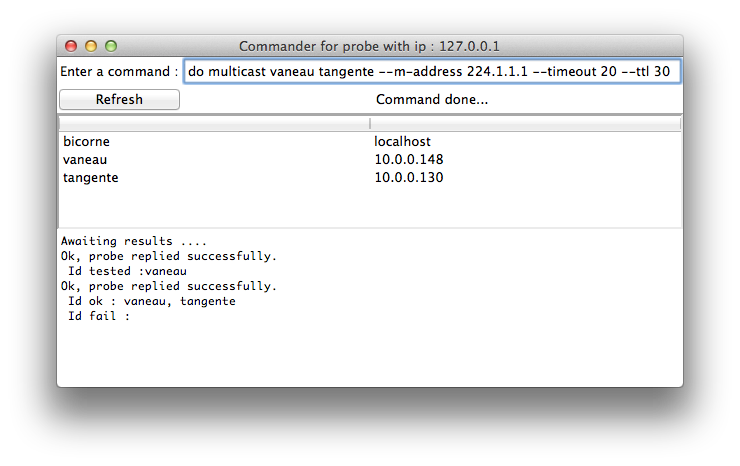
\includegraphics[width=\linewidth]{img/commander.png}
\end{minipage}
\hfill
\begin{minipage}[c]{0.5\linewidth}
\begin{description}
\item[ligne d'entrée] permet de donner des commandes à la sonde
\item[ligne de statut] permet d'afficher le status de la commande exécutée
\item[bouton rafraichir] permet de rafraichir les sondes connues en les demandant au serveur commandé
\item[affichage des sondes] tableau id | adresse IP des sondes connues
\item[panneau résultats] affiche les résultats des tests lancés
\end{description}
\end{minipage}
\end{figure}
\FloatBarrier

Les commandes supportés sont les suivantes :
\begin{description}
\item[add ip] ajoute la sonde d'adresse IP 'ip' à notre réseau de sondes. On peut ensuite effectuer des tests dessus.
\item[remove id] supprime la sonde id du réseau. Supprimer la sonde commandée permet de la retirer du réseau.
\item[do testname testoptions] effectue le test 'testname' sur la sonde commandée avec les options testoptions. Les options sont de la forme option=valeur.
\end{description}
\vspace{2ex}
\textbf{Affichage des résultats}

Les résultats sont automatiquement affichés lorsqu'ils sont disponibles sur la sonde commandée dans le panneau prévu à cet effet.


\subsubsection{Exemples}
% Mettre un capture d'écran avec des meilleurs noms
\subsubsection*{Ajouter des sondes}
\texttt{add 10.0.0.148}\\
\indent\texttt{add 10.0.0.130}

\subsubsection*{Effectuer des tests}
\texttt{do unicast tangente --port 5611 --protocol tcp}\\
\indent\texttt{do unicast vaneau --timeout 2 --protocol udp}\\
\indent\texttt{do broadcast --port 7267 --timeout 3.5 }\\
\indent\texttt{do multicast vaneau tangente --port 12456 --timeout 3.4 --ttl 20 -ma 224.4.6.6}\\
\indent\texttt{do empty}

\section{Architecture et fonctionnement}


\subsection{Architecture}

On représente ci-dessous l'organisation globale des différents threads qui composent les sondes du réseau.
Les conventions de représentations sont les suivantes :
\begin{figure}[!ht]
\centering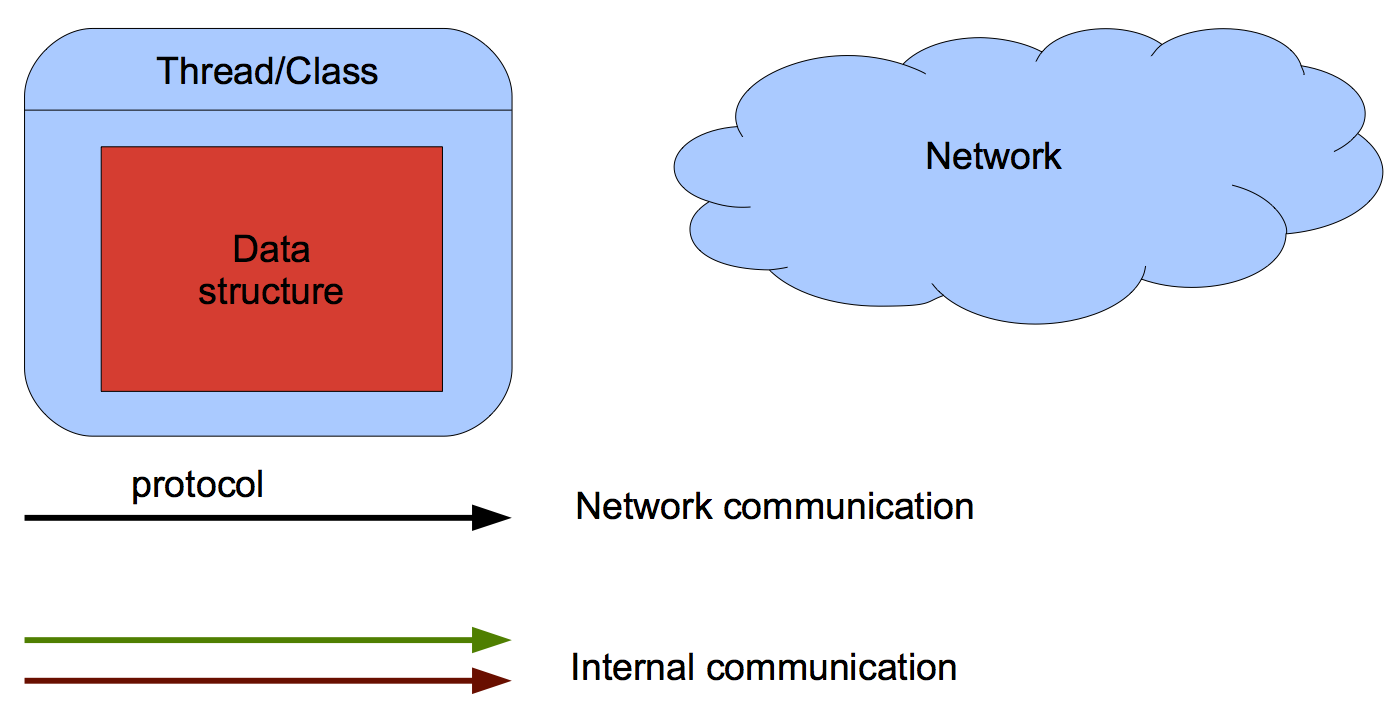
\includegraphics[width=\linewidth]{img/graphLegend.png}
\caption{Légende}
\end{figure}



Une sonde est composé dans sa version la plus simple de 3 threads et de 3 structures de stockage de données.
\begin{itemize}
\item L'objet \cd{ProbeStorage} contient les sondes du réseau (Id, IP), ainsi que les objets représentant les connexions HTTP vers ces sondes.
\item Le thread \cd{Client} gère une file de messages. Il utilise les connexions du \cd{probestorage} pour les envoyer au fur et à mesure.
\item Le thread \cd{Server} écoute les requêtes HTTP sur le port de communication interne des sondes et transforme les messages reçus en actions qu'il stocke dans une file d'attente.
\item Le thread \cd{ActionMan} dépile les actions dans l'ordre de priorité et les exécute.
\end{itemize}
\begin{figure}[!ht]
\begin{minipage}[c]{0.3\linewidth}

Le commander est un thread à part qui peut même être lancé à partir d'une machine sur laquelle ne tourne aucune sonde. Ce programme prend en entrée une machine (adresse IP) sur laquelle fonctionne une sonde avec qui communiquer. Il utilise cette sonde pour connaitre le réseau et déclencher des tests.
\end{minipage}
\hfill
\begin{minipage}[c]{0.65\linewidth}

\centering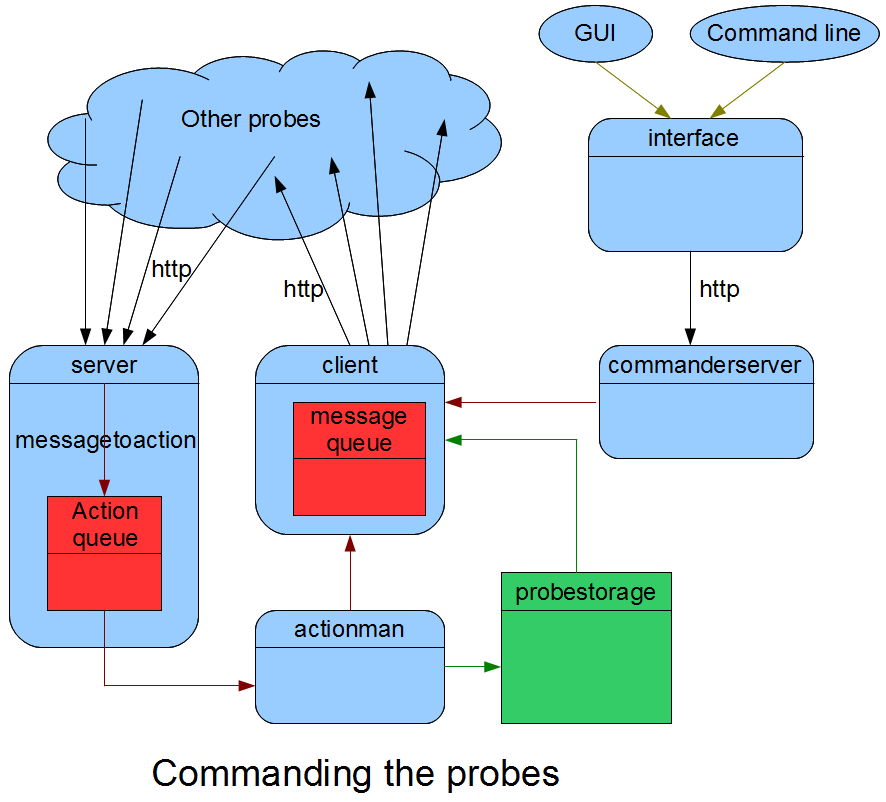
\includegraphics[width=\linewidth]{img/graphCommander.png}
\caption{Fonctionnement d'une sonde}
\end{minipage}
\end{figure}
\FloatBarrier

Les threads mis en jeu sont :
\begin{description}
\item[Le thread \cd{Interface} graphique (GUI) ou en ligne de commande (CLI)], elle est à la fois le serveur et le client qui permet de communiquer avec une sonde commandée.
\item[Le thread \cd{CommanderServer}] tourne sur la sonde et écoute les requêtes HTTP sur le port de communication "commander" des sondes. Il réagit immédiatement aux messages reçu du commander.
\end{description}
Lors de l'exécution d'un test, un thread particulier, est lancé par les sondes. Le thread \cd{ActionMan} est bloqué jusqu'à l'arrêt du test.
\begin{itemize}
\item \cd{TestManager} pour la sonde qui exécute le test.
\item \cd{TestResponder} pour les sondes qui réagissent au test.
\end{itemize}

\begin{figure}[!ht]
\centering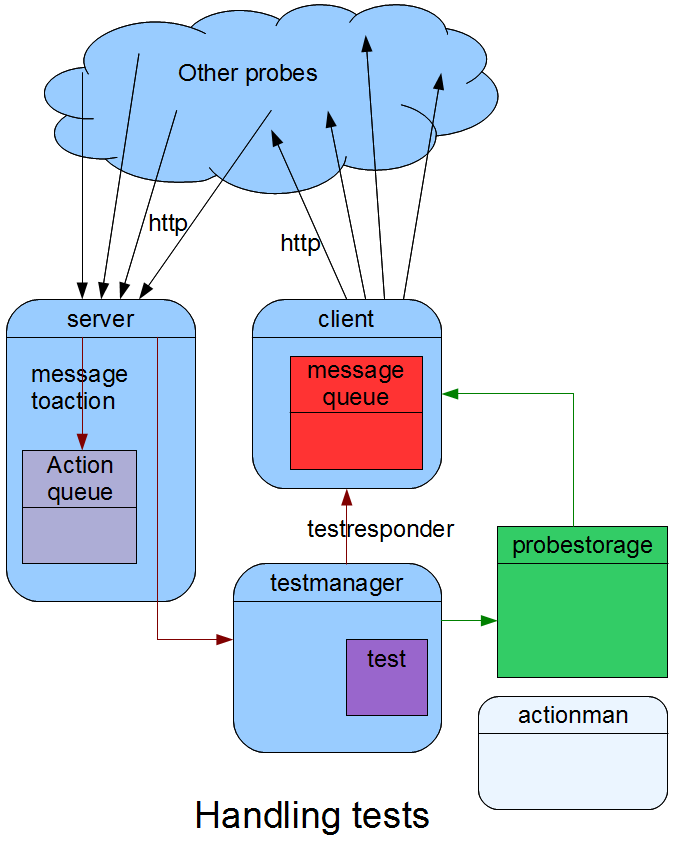
\includegraphics[width=0.8\linewidth]{img/graphTest.png}
\caption{Fonctionnement alternatif lors d'un test}
\end{figure}

\FloatBarrier


\subsection{Fonctionnement}

\subsubsection{Ajout d'une sonde au réseau}

Détail des étapes lors de l'ajout d'une sonde au réseau :
\begin{itemize}
\item L'utilisateur lance une commande "add" : \texttt{add 10.0.0.130}
\item L'interface crée un requête HTTP "POST" contenant l'IP de la machine sur laquelle tourne la sonde à ajouter.
\item A la réception de cette requête, le \texttt{CommanderServer} sur lequel est branché l'interface envoie une requête "GET" à l'adresse IP désirée et attend la réponse de la sonde.
\item La nouvelle sonde (si elle existe bien) renvoie son ID à la réception de la requête "GET"
\item Le \texttt{CommanderServer} demande alors au \texttt{client} d'envoyer à toute les ondes (y compris celle sur laquelle il tourne) le message "Add" avec le flag "Hello" à True et les paramètres de la nouvelle sonde.
\item Le client dépile les messages "Add" et les envoie au fur et à mesure.
\item Les serveurs des sondes du réseau, à la réception de ce message, empilent une action "Add" avec flag "hello".
\end{itemize}

\begin{figure}[!ht]
\centering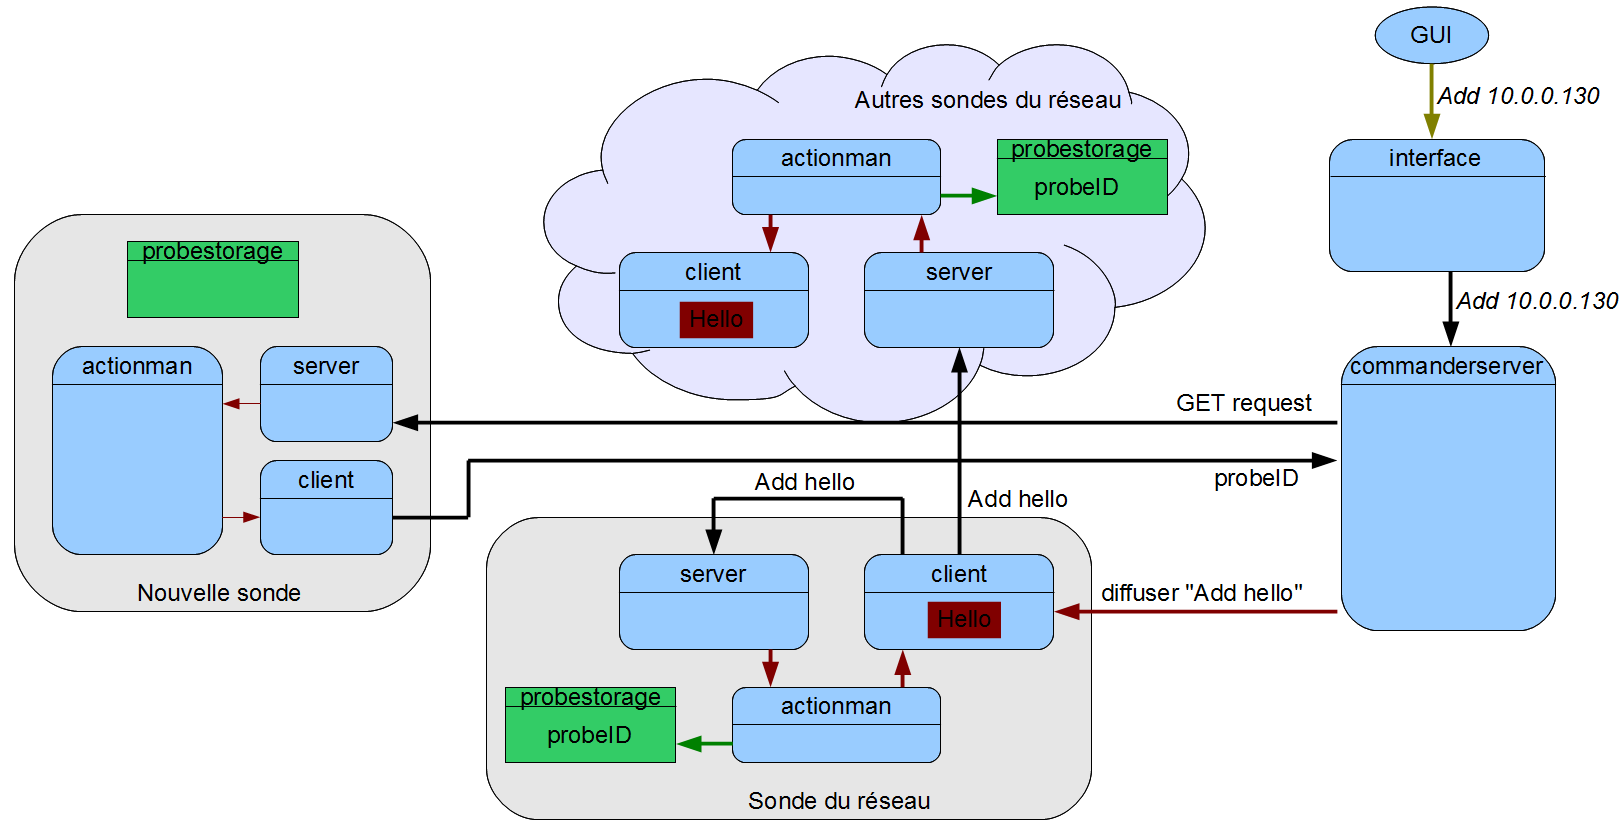
\includegraphics[width=0.8\linewidth]{img/graphAdd1.png}
\caption{Ajout d'une sonde - Etape 1}
\end{figure}

\begin{itemize}
\item Les \texttt{ActionMan} de chaque sonde dépilent cette action et l'exécutent : Ils ajoutent la nouvelle sonde dans le \texttt{ProbeStorage} et chargent le \texttt{client} d'envoyer à cette nouvelle sonde un message "Hello".
\item Le client s'exécute.
\item Le serveur de la nouvelle sonde empile une action "Add" sans flag "hello" pour chaque message "Hello" qu'elle reçoit.
\item A la lecture de ces "Add" de toutes les sondes du réseaux, l'\texttt{ActionMan} de la nouvelle sonde se constitue un répertoire complet des sondes du réseau.
\end{itemize}

\begin{figure}[!ht]
\centering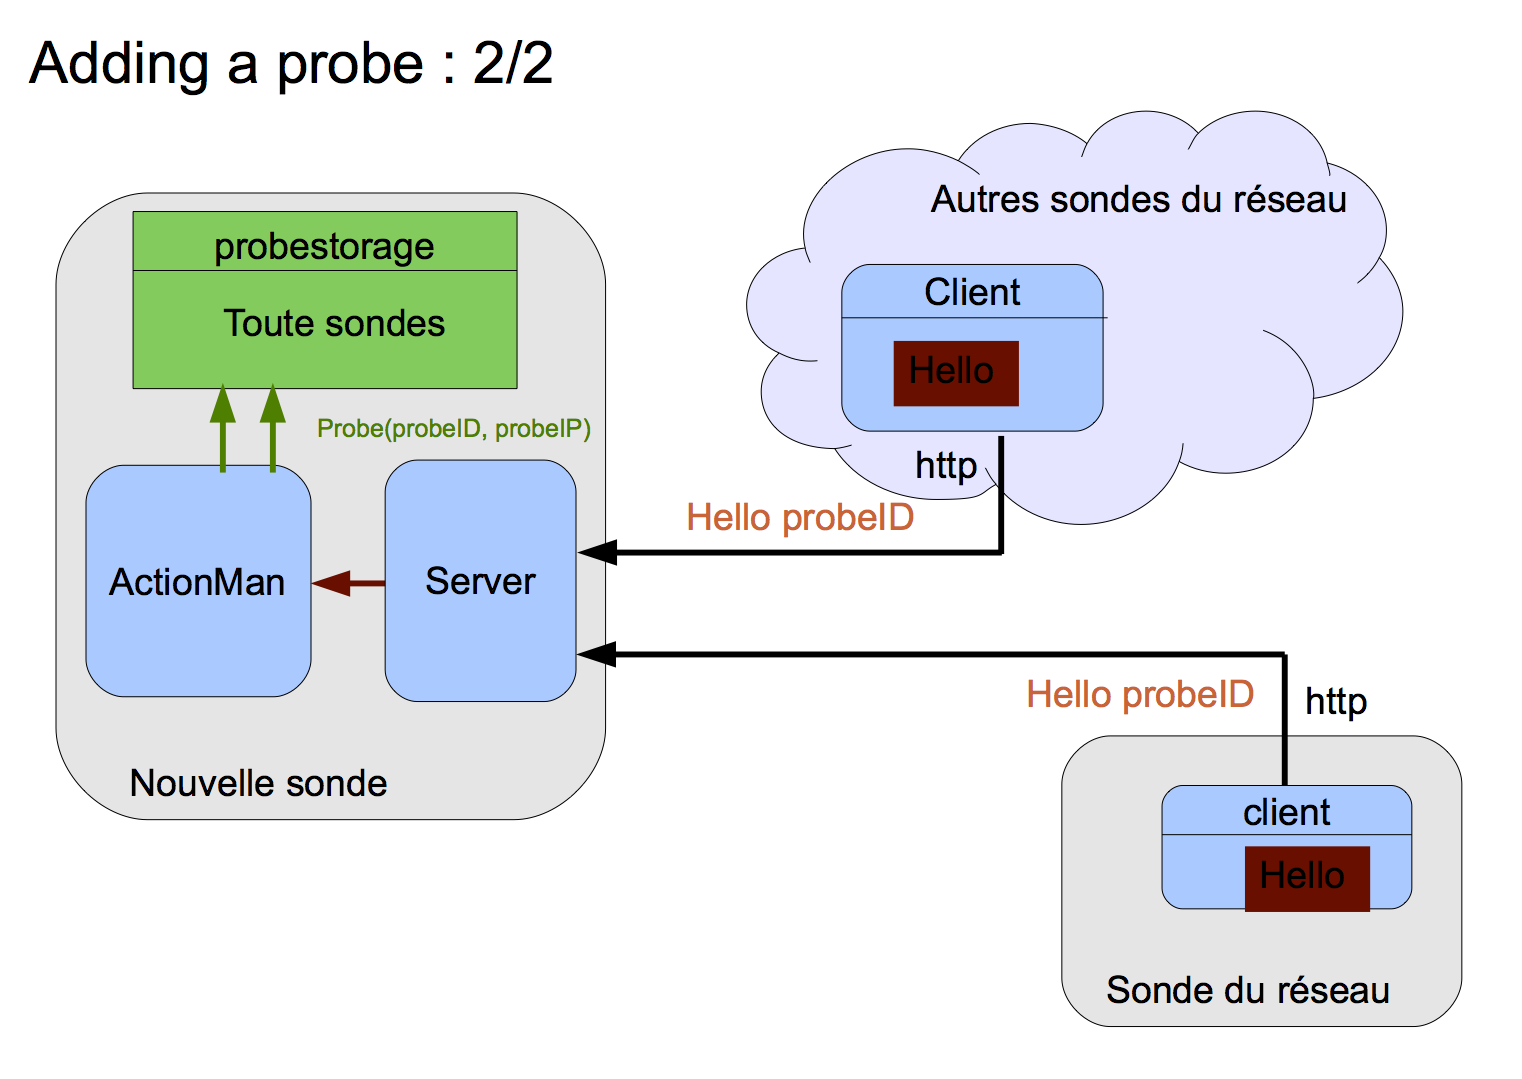
\includegraphics[width=0.6\linewidth]{img/graphAdd2.png}
\caption{Ajout d'une sonde - Etape 2}
\end{figure}

\FloatBarrier



\subsubsection{Exécution d'un test}

Détail des étapes lors de l'exécution d'un test :

\begin{itemize}
\item L'utilisateur lance une commande "do" : \texttt{do unicast tangente}
\item Le \texttt{CommanderServer} empile une action correspondant dans la pile du \texttt{Server}.
\item L'\texttt{ActionMan}, à la lecture de cette action lance le test et bloque jusqu'à la fin de celui-ci. La main est laissée aux fonctions du \texttt{TestManager}.
\item Le \texttt{TestManager} lit les options du test et envoie aux sondes concernées un message "Prepare" contenant les options du test.

\end{itemize}
\begin{figure}[!ht]
\centering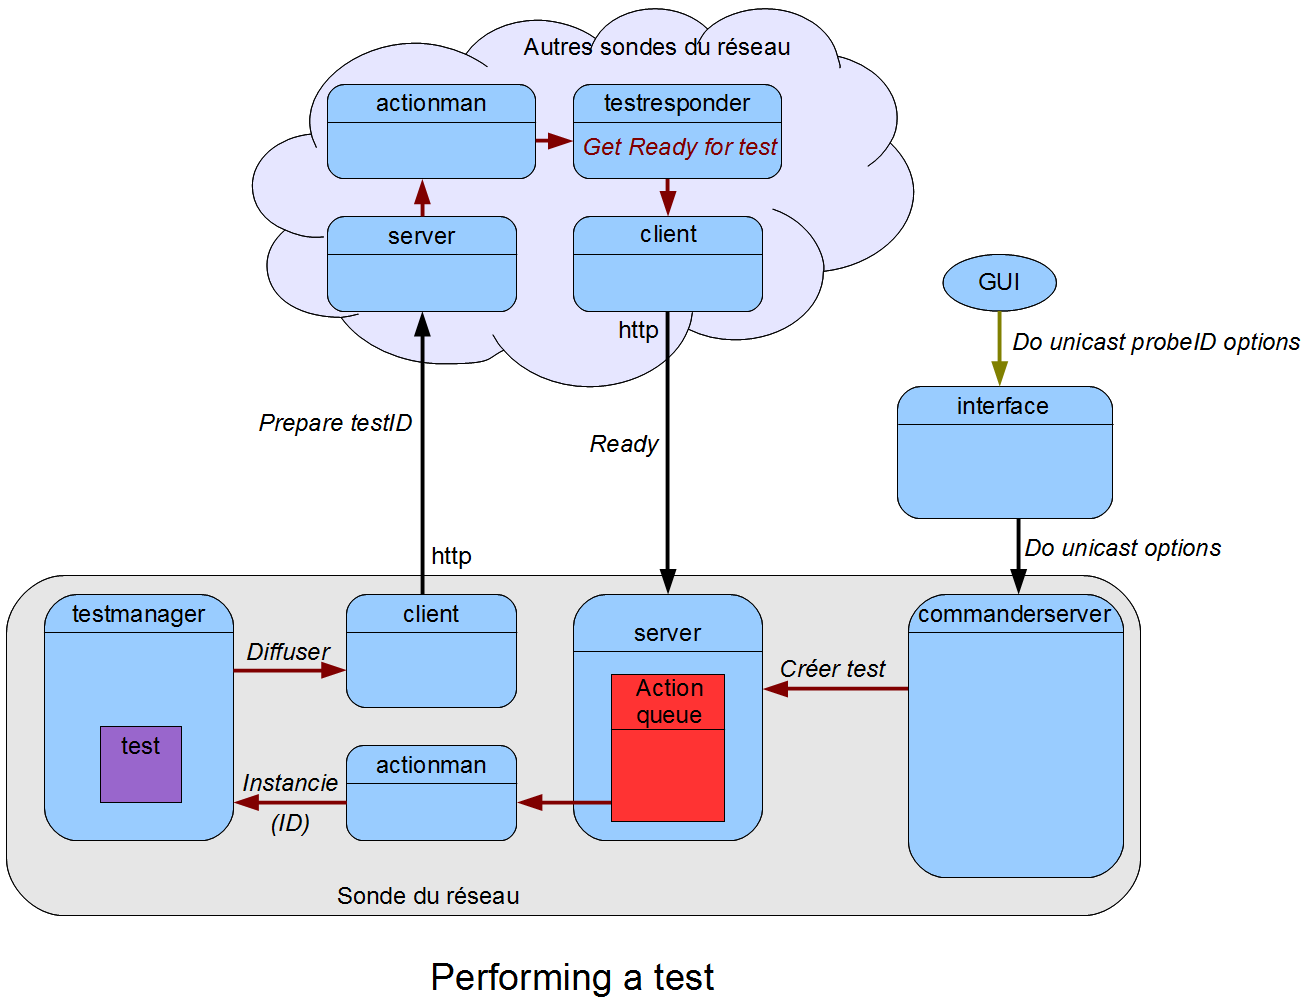
\includegraphics[width=0.8\linewidth]{img/graphTest1.png}
\caption{Exécution d'un test - Etape 1}
\end{figure}

\begin{itemize}
\item Les serveurs de ces sondes transforme ce message en action.
\item L'\texttt{ActionManager} de ces sondes bloque et cède la main aux fonctions du \texttt{TestResponder}.
\item Ce dernier effectue les préparatifs pour le test puis envoie, via le \texttt{Client} un message "Ready" à la sonde qui a initié le test.
\item Le \texttt{TestManager} de cette sonde attend de recevoir les messages "Ready" de toute les sondes cibles. En cas d'erreur ou de non réception d'un des "Ready", elle renvoie à tous un message "Abort".
\item Le test est effectué par la sonde initiatrice.
\item Le \texttt{TestManager} envoie un message "Over" à toute les sondes participant au test.
\item Ces dernières répondent un message "Result" contenant les résultats qu'elles ont obtenus.
\item A la réception de tout les résultats, le \texttt{TestManager} construit un rapport qu'il retourne au \texttt{CommanderServer}, lequel était bloqué jusqu'à la réception de ce rapport.
\item Le \texttt{CommanderServer} répond à l'interface qui met à jour son affichage.
\end{itemize}

\begin{figure}[!ht]
\centering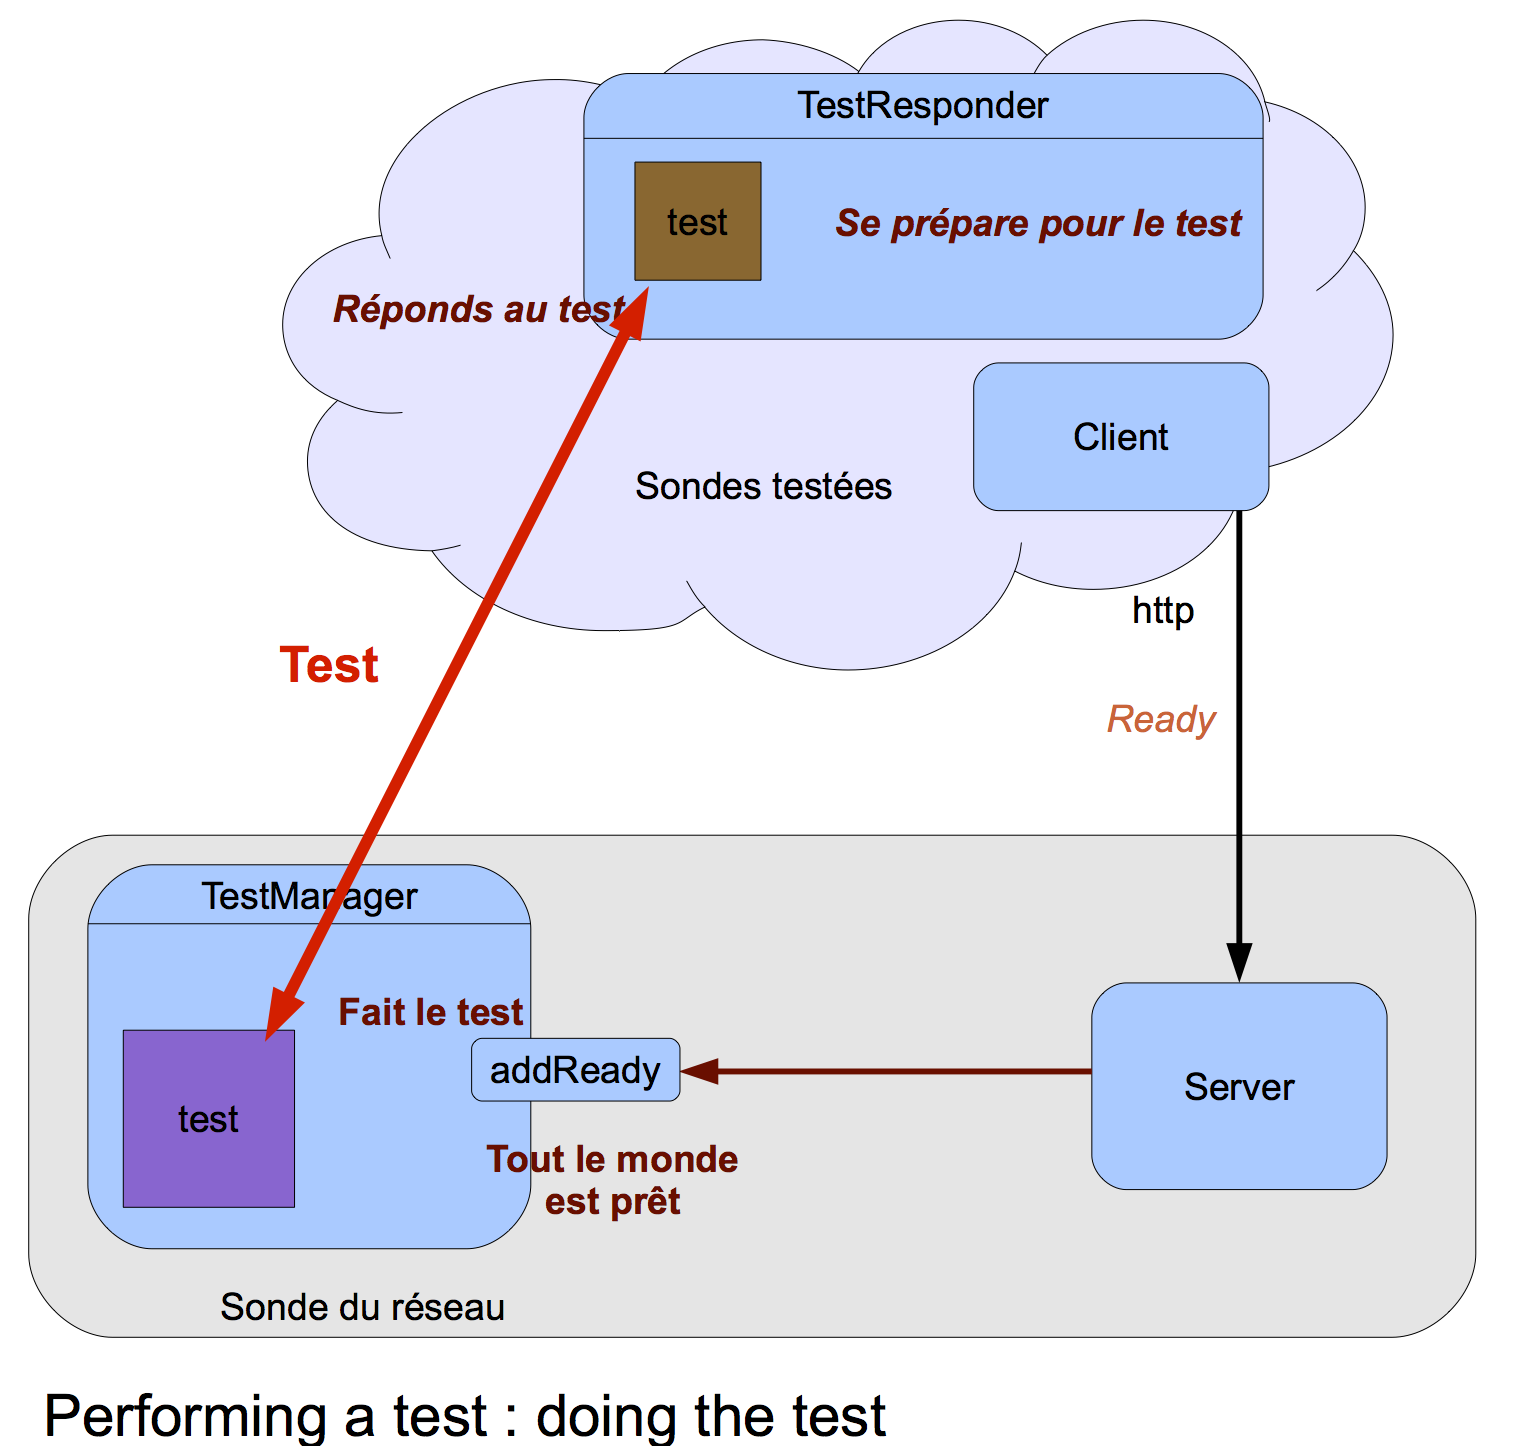
\includegraphics[width=0.8\linewidth]{img/graphTest2.png}
\caption{Exécution d'un test - Etape 2}
\end{figure}

\begin{itemize}
\item Le \texttt{TestManager} envoie un message "Over" à toute les sonde participant au test.
\item Ces dernières répondent un message "Result" contenant les résultats qu'elles ont obtenus.
\item A la réception de tout les résultats, le \texttt{TestManager} construit un rapport qu'il retourne au \texttt{CommanderServer}, lequel était bloqué jusqu'à la réception de ce rapport.
\item Le \texttt{CommanderServer} Répond à l'interface qui met à jour son affichage.
\end{itemize}

\begin{figure}[!ht]
\centering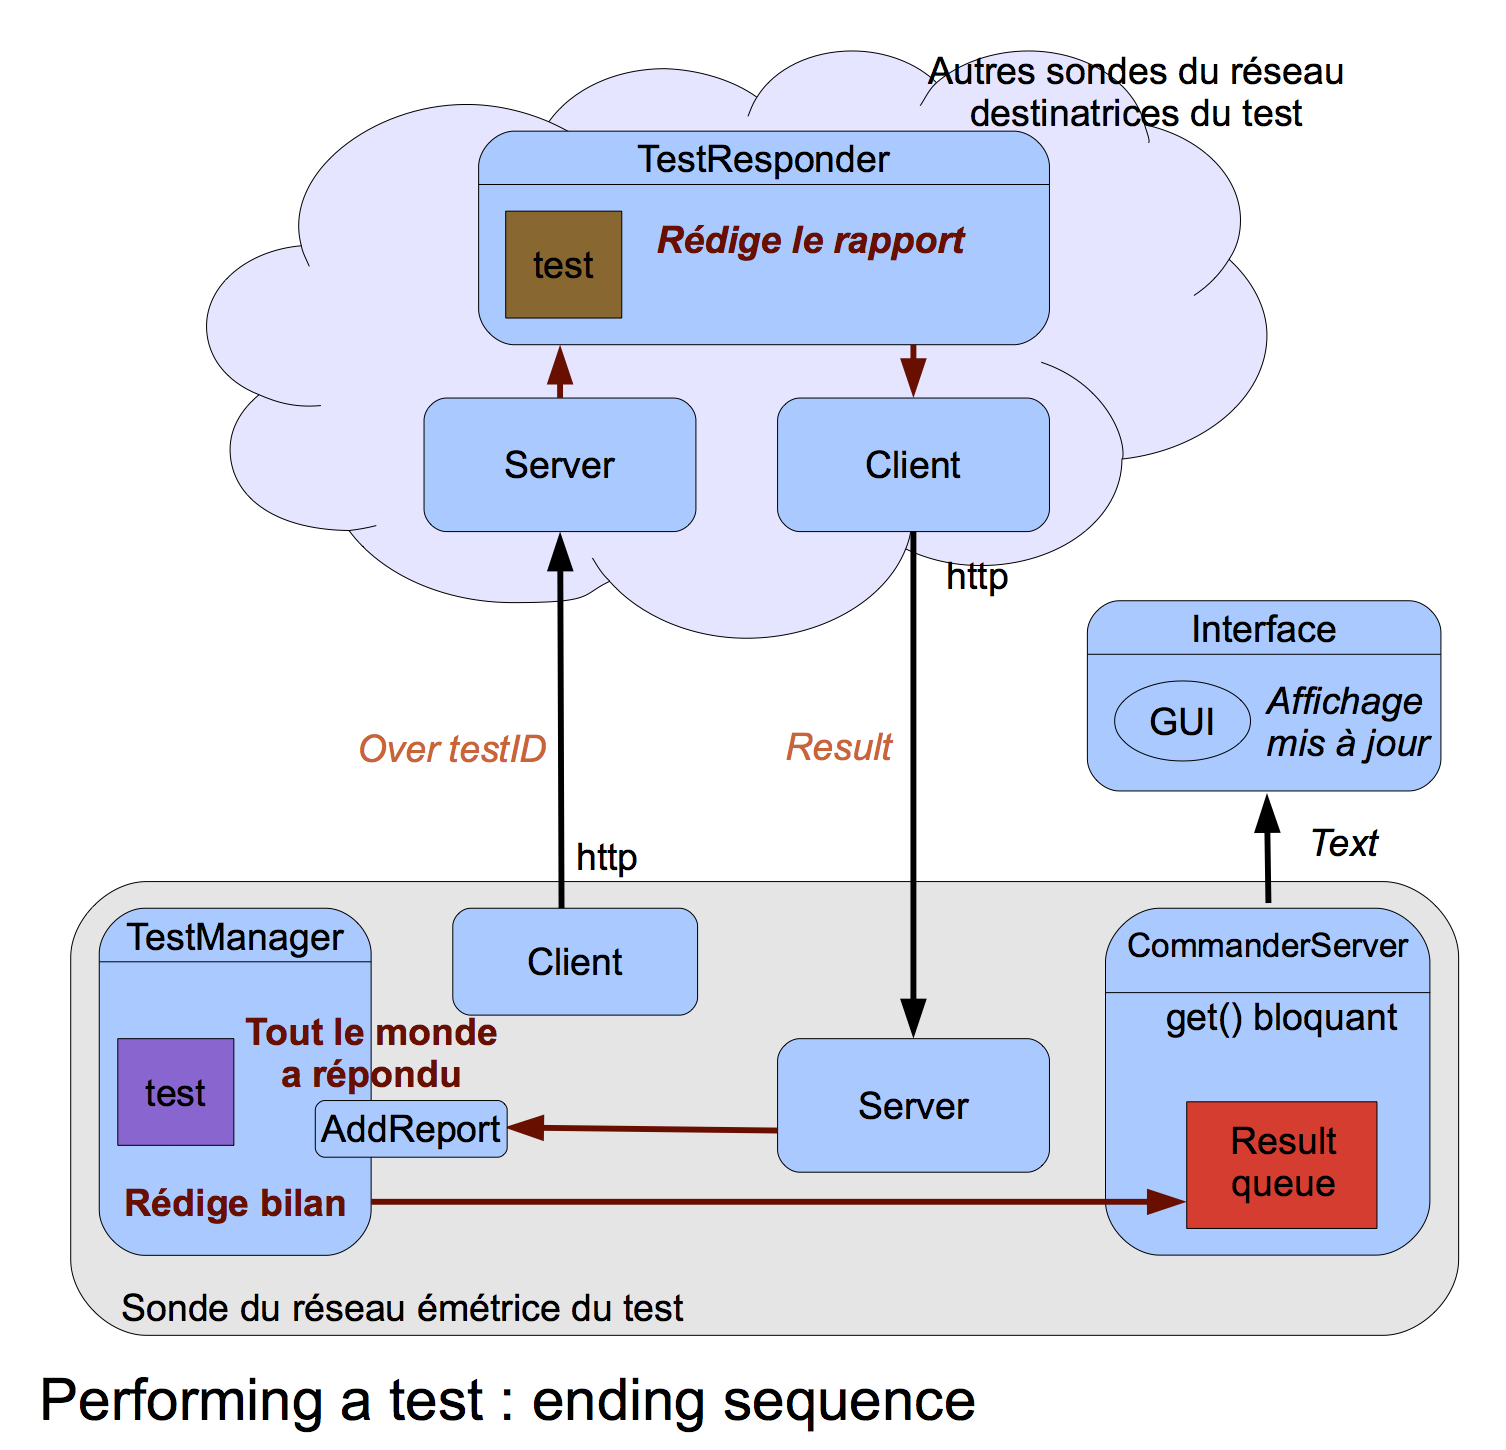
\includegraphics[width=0.8\linewidth]{img/graphTest3.png}
\caption{Exécution d'un test - Etape 3}
\end{figure}

\FloatBarrier

\subsection{Tables de fonctionnement}

\begin{center}
\begin{tabular}{|l|l|c|l|}
\hline
\cd{Server} & \multicolumn{3}{|c|}{\cd{ActionMan}} \\
\hline
\textbf{Message} & \textbf{Action} & & \\
\hline
Add & Add & $\longrightarrow$ & Ajout dans la table / Message "Hello" si nécessaire\\
\hline
Hello & Add & $\longrightarrow$ & Ajout dans la table\\
\hline
\multirow{2}{*}{Bye} & Remove & $\longrightarrow$ & Supprime la sonde de la table\\
\cline{2-4}
 & Quit & $\longrightarrow$ & Diffuse un message "Bye" / Coupe toute les connexions sauf la sienne\\
\hline
Prepare & Prepare & $\longrightarrow$ & Lance le test / Bloque jusqu'à la fin du test \\
\hline
\end{tabular}
\end{center}

\begin{center}
\begin{tabular}{|l|l|}
\hline
\multicolumn{2}{|c|}{\cd{CommanderServer}} \\
\hline
\textbf{Message} & \\
\hline
Add & Requête "GET" vers la nouvelle sonde pour connaitre son ID / Diffuse un message "Add" \\
\hline
Delete & Envoie un message "Bye"\\
\hline
Do & Met une action "Do" dans le pile d'actions\\
\hline
\end{tabular}
\end{center}

%appendice éventuel
\clearpage
\rhead{Annexe}
\renewcommand{\appendixpagename}{\centering{Annexe : Liste des fonctions Scilab}}
\renewcommand{\labelitemi}{$\bullet$}
\renewcommand{\labelitemiii}{$\cdot$}
\renewcommand{\labelitemii}{$\diamond$}
\renewcommand{\labelitemiv}{$\ast$}
\begin{appendices}
\section{Organisation du code}

\fbox{
\begin{minipage}{\linewidth}
\textbf{Thread}
\begin{itemize}
\item \cd{Server}
	\begin{itemize}
	\item \cd{Listener(ThreadingMixIn, HTTPServer, Thread)}
		\begin{itemize}
		\item \cd{RequestHandler(SimpleHTTPRequestHandler)}
		\end{itemize}
	\end{itemize}

\item \cd{CommanderServer}
	\begin{itemize}
	\item \cd{Listener(ThreadingMixIn, HTTPServer, Thread)}
		\begin{itemize}
		\item \cd{RequestHandler(SimpleHTTPRequestHandler)}
		\end{itemize}
	\end{itemize}

\item \cd{Client}
\item \cd{ActionMan}
\end{itemize}
\end{minipage}
}

\fbox{
\begin{minipage}{\linewidth}
\textbf{Object}\\
~
\hfill
	\fbox{
	\begin{minipage}{0.3\linewidth}
		\cd{Message} 
		\begin{itemize}
		\item \cd{Add}
		\item \cd{Hello}
		\item \cd{Bye}
		\item \cd{TestMessage}
		\begin{itemize}
			\item \cd{Prepare}
			\item \cd{TesterMessage}
				\begin{itemize}
				\item \cd{Over}
				\item \cd{Abort}
				\end{itemize}
			\item \cd{TesteeMessage}
				\begin{itemize}
				\item \cd{Ready}
				\item \cd{Result}
				\end{itemize}
			\end{itemize}
		\end{itemize}
		\cd{Probe}
		\cd{ProbeStorage}
	\end{minipage}
	}
	\hfill
	\fbox{
	\begin{minipage}{0.2\linewidth}
	\cd{Action} 
		\begin{itemize}
		\item \cd{Add}
		\item \cd{Remove}
		\item \cd{Do}
		\item \cd{Prepare}
		\item \cd{Quit}
		\end{itemize}
	\end{minipage}
	}
	\hfill
	\fbox{
	\begin{minipage}{0.3\linewidth}
	\begin{itemize}
	\item \cd{Test}
		\begin{itemize}
		\item \cd{Unicast}
		\item \cd{Multicast}
		\item \cd{Broadcast}
		\item \cd{Empty}
		\end{itemize}
	
	\item \cd{TestManager}
	\item \cd{TestResponder}
	\end{itemize}
	\end{minipage}
	}
	\hfill
	\fbox{
	\begin{minipage}{0.2\linewidth}
	\cd{Interface}
		\begin{itemize}
		\item \cd{Gui}
		\item \cd{Cli}
		\end{itemize}
	\cd{Parser}
	\end{minipage}
	}
	\hfill
	\fbox{
	\begin{minipage}{0.23\linewidth}
	\begin{itemize}
		\item \cd{Consts}
		\item \cd{Params}
		\item \cd{Identification}
	\end{itemize}
	\end{minipage}
	}
	\hfill
	\fbox{
	\begin{minipage}{0.25\linewidth}
	\cd{Exception}
		\begin{itemize}
		\item \cd{NoSuchProbe}
		\item \cd{TestInProgress}
		\item \cd{NoSuchCommand}
		\end{itemize}
	
	\end{minipage}
	}
	\hfill
	~
\end{minipage}
}
\end{appendices}
\end{document}
